\documentclass{article}
\usepackage[paperwidth=7.35in,paperheight=6.25in,margin=0in]{geometry}
\usepackage{amsmath}
\usepackage{tikz}
\usetikzlibrary{arrows.meta,calc}
\pagestyle{empty}

\begin{document}
\noindent
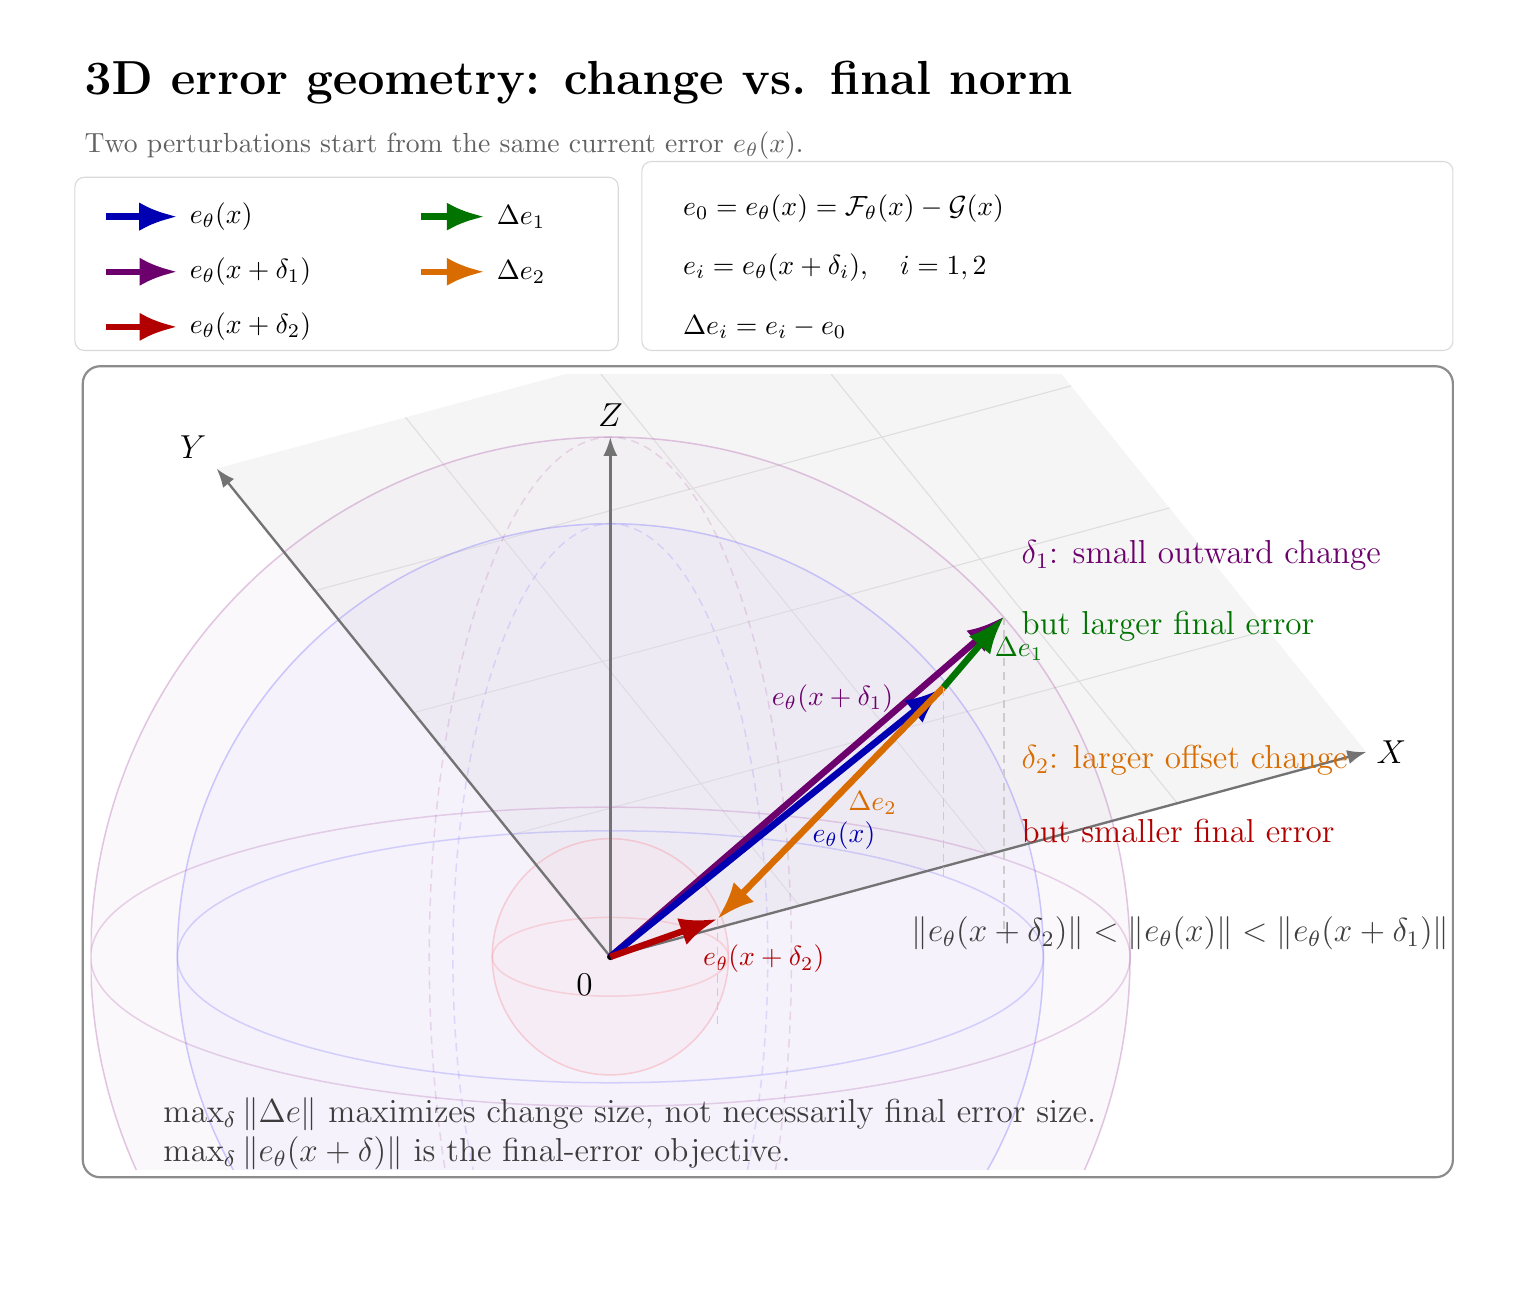
\begin{tikzpicture}[
  x=1mm,y=1mm,
  >=Latex,
  font=\sffamily,
  panel/.style={draw=black!45, rounded corners=2.2mm, line width=0.8pt, fill=white},
  axis/.style={->, draw=black!55, line width=0.85pt},
  gridline/.style={draw=black!13, line width=0.4pt},
  eold/.style={->, draw=blue!70!black, line width=2.4pt},
  enewone/.style={->, draw=violet!85!black, line width=2.35pt},
  enewtwo/.style={->, draw=red!70!black, line width=2.35pt},
  deone/.style={->, draw=green!45!black, line width=2.35pt},
  detwo/.style={->, draw=orange!85!black, line width=2.35pt},
  guide/.style={draw=black!20, densely dashed, line width=0.45pt},
  formula/.style={font=\normalsize, align=left, anchor=west},
  note/.style={font=\large, align=left, anchor=west}
]
\path[use as bounding box] (0,0) rectangle (186,158);

% Header
\node[font=\LARGE\bfseries, anchor=west] at (6,151)
  {3D error geometry: change vs. final norm};
\node[font=\normalsize, text=black!62, anchor=west] at (6,143)
  {Two perturbations start from the same current error $e_\theta(x)$.};

% Legend, outside the 3D panel so it does not cover the axes.
\fill[white, opacity=0.94] (6,117) rectangle (75,139);
\draw[black!15, rounded corners=1.2mm] (6,117) rectangle (75,139);
\draw[eold] (10,134) -- ++(9,0) node[right, black, font=\normalsize] {$e_\theta(x)$};
\draw[enewone] (10,127) -- ++(9,0) node[right, black, font=\normalsize] {$e_\theta(x+\delta_1)$};
\draw[enewtwo] (10,120) -- ++(9,0) node[right, black, font=\normalsize] {$e_\theta(x+\delta_2)$};
\draw[deone] (50,134) -- ++(8,0) node[right, black, font=\normalsize] {$\Delta e_1$};
\draw[detwo] (50,127) -- ++(8,0) node[right, black, font=\normalsize] {$\Delta e_2$};

% Definitions, deliberately below the title so nothing overlaps.
\fill[white, opacity=0.92] (78,117) rectangle (181,141);
\draw[black!15, rounded corners=1.2mm] (78,117) rectangle (181,141);
\node[formula] at (82,135)
  {$e_0=e_\theta(x)=\mathcal F_\theta(x)-\mathcal G(x)$};
\node[formula] at (82,127.5)
  {$e_i=e_\theta(x+\delta_i),\quad i=1,2$};
\node[formula] at (82,120)
  {$\Delta e_i=e_i-e_0$};

% Main panel
\draw[panel] (7,12) rectangle (181,115);

% Projected 3D basis:
% X=(15,4), Y=(-8,10), Z=(0,12)
\coordinate (O)  at (74,40);
\coordinate (X)  at ($(O)+(96,26)$);
\coordinate (Y)  at ($(O)+(-50,62)$);
\coordinate (Z)  at ($(O)+(0,66)$);
\coordinate (XY) at ($(O)+(46,88)$);

% Projected points:
% e0=(3.3,0.9,1.0)
% e1 is reached by a small outward change about 10-20 degrees from e0
% e2=(0.8,-0.2,0.3), a much shorter final error after a large opposite change
\coordinate (E0) at ($(O)+(42.3,34.2)$);
\coordinate (N1) at ($(O)+(50.0,43.2)$);
\coordinate (N2) at ($(O)+(13.6,4.8)$);

\begin{scope}
  \clip (8,13) rectangle (180,114);
  % Projected floor plane.
  \fill[black!4] (O) -- (X) -- (XY) -- (Y) -- cycle;
  \foreach \t in {0.25,0.5,0.75} {
    \draw[gridline] ($(O)!\t!(X)$) -- ($(Y)!\t!(XY)$);
    \draw[gridline] ($(O)!\t!(Y)$) -- ($(X)!\t!(XY)$);
  }

  % Transparent norm shells centered at the origin. These are not endpoint markers.
  \fill[red!14, opacity=0.20] (O) circle[radius=15mm];
  \draw[red!50, opacity=0.42, line width=0.55pt] (O) circle[radius=15mm];
  \draw[red!50, opacity=0.35, line width=0.55pt] (O) ellipse[x radius=15mm,y radius=5mm];

  \fill[blue!15, opacity=0.18] (O) circle[radius=55mm];
  \draw[blue!55, opacity=0.40, line width=0.55pt] (O) circle[radius=55mm];
  \draw[blue!55, opacity=0.32, line width=0.55pt] (O) ellipse[x radius=55mm,y radius=16mm];
  \draw[blue!55, opacity=0.24, densely dashed, line width=0.55pt] (O) ellipse[x radius=20mm,y radius=55mm];

  \fill[violet!16, opacity=0.16] (O) circle[radius=66mm];
  \draw[violet!60, opacity=0.36, line width=0.55pt] (O) circle[radius=66mm];
  \draw[violet!60, opacity=0.28, line width=0.55pt] (O) ellipse[x radius=66mm,y radius=19mm];
  \draw[violet!60, opacity=0.22, densely dashed, line width=0.55pt] (O) ellipse[x radius=23mm,y radius=66mm];
\end{scope}

% Axes
\draw[axis] (O) -- (X) node[right, font=\large] {$X$};
\draw[axis] (O) -- (Y) node[above left, font=\large] {$Y$};
\draw[axis] (O) -- (Z) node[above, font=\large] {$Z$};
\fill[black] (O) circle[radius=1.2pt] node[below left=1mm, font=\large] {$0$};

% Vectors: all delta arrows connect exactly from e0 endpoint to the corresponding final endpoint.
\draw[enewone] (O) -- (N1)
  node[pos=0.76, left=0.5mm, font=\normalsize, text=violet!85!black] {$e_\theta(x+\delta_1)$};
\draw[eold] (O) -- (E0)
  node[pos=0.56, below right=0.4mm, font=\normalsize, text=blue!70!black] {$e_\theta(x)$};
\draw[enewtwo] (O) -- (N2)
  node[pos=0.72, below right=0.4mm, font=\normalsize, text=red!70!black] {$e_\theta(x+\delta_2)$};
\draw[deone] (E0) -- (N1)
  node[pos=0.54, right=0.8mm, font=\normalsize, text=green!45!black] {$\Delta e_1$};
\draw[detwo] (E0) -- (N2)
  node[pos=0.50, right=0.7mm, font=\normalsize, text=orange!85!black] {$\Delta e_2$};

% Light guides to clarify endpoints without drawing endpoint circles.
\draw[guide] (E0) -- ($(E0)+(0,-24)$);
\draw[guide] (N1) -- ($(N1)+(0,-40)$);
\draw[guide] (N2) -- ($(N2)+(0,-14)$);

% Interpretation labels
\node[note, text=violet!85!black] at (125,91) {$\delta_1$: small outward change};
\node[note, text=green!45!black] at (125,82) {but larger final error};
\node[note, text=orange!85!black] at (125,65) {$\delta_2$: larger offset change};
\node[note, text=red!70!black] at (125,56) {but smaller final error};
\node[note, text=black!75] at (111,43)
  {$\|e_\theta(x+\delta_2)\|<\|e_\theta(x)\|<\|e_\theta(x+\delta_1)\|$};

% Bottom conclusion
\node[font=\large, anchor=west, text=black!76] at (16,20)
  {$\max_\delta \|\Delta e\|$ maximizes change size, not necessarily final error size.};
\node[font=\large, anchor=west, text=black!76] at (16,15)
  {$\max_\delta \|e_\theta(x+\delta)\|$ is the final-error objective.};

\end{tikzpicture}
\end{document}
